4. $\cfrac{(5x^2+6x+1)(x-2)^2}{x-4}\geqslant0\Leftrightarrow\cfrac{5\left(x+\cfrac{1}{5}\right)(x+1)(x-2)^2}{x-4}\geqslant0.$ Применив метод интервалов, найдём ответ:
\begin{figure}[ht!]
\center{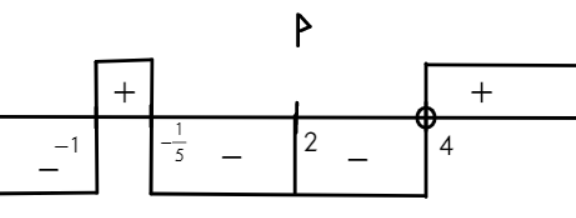
\includegraphics[scale=0.45]{int4.png}}
\end{figure}
$x\in\left[-1;-\cfrac{1}{5}\right]\cup\{2\}\cup(4;+\infty).$\newpage\noindent
